%!TEX root = ../these.tex

\chapter{
  Точный алгоритм решения
  обобщенной задачи коммивояжера
  с ограничениями предшествования
  PCGTSP
}
\label{ch:pcgtsp}

\begin{figure}
  \centering
  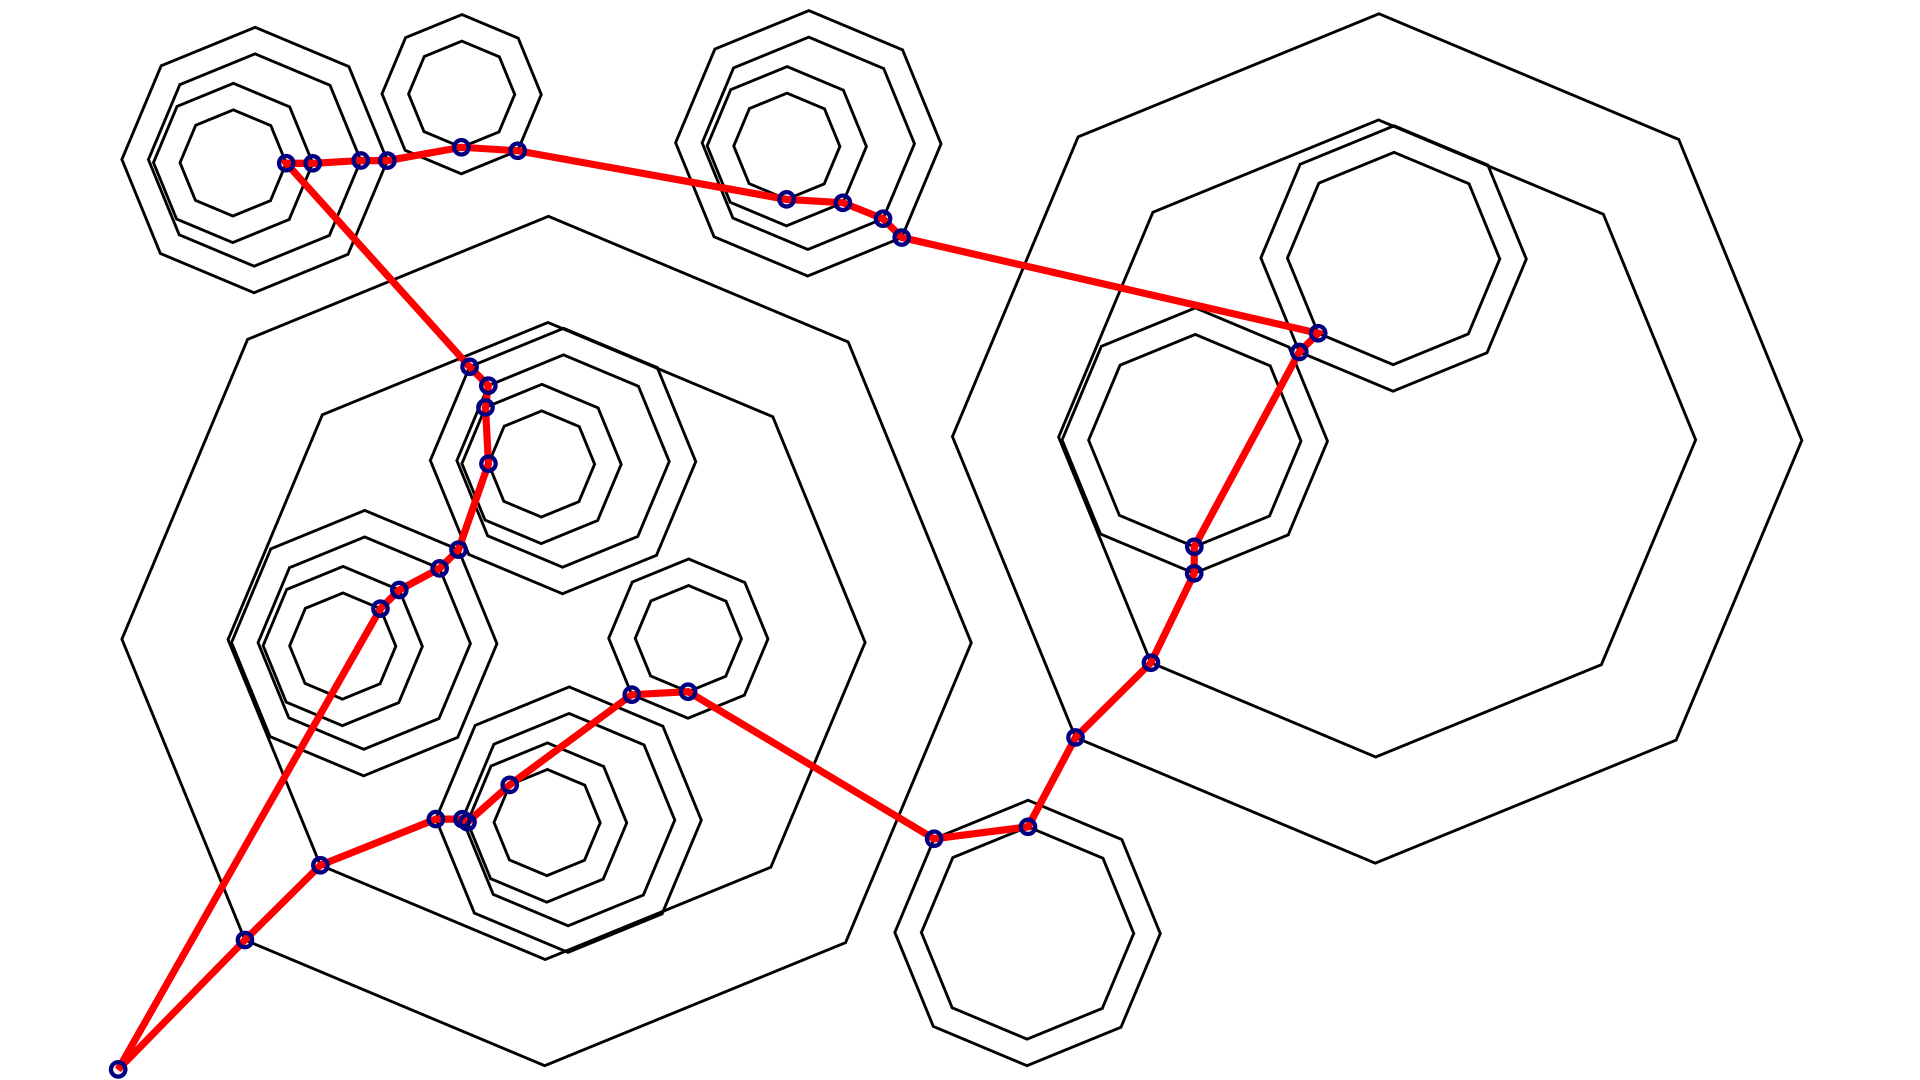
\includegraphics[width=0.95\textwidth]{34.png}
  \caption{Пример решения задачи PCGTSP, полученного эвристикой PCGLNS}
  \label{fig:pcgtsp.svg}
\end{figure}

%!TEX root = ../these.tex

\section{%
Использование модели обобщенной задачи коммивояжера
с ограничениями предшествования
PCGTSP
для формализации задачи маршрутизации
}
\label{sec:pcgtsp.intro}

Обобщенная задача коммивояжера
(Generalized Traveling Salesman Problem, GTSP)
-- широко известная задача комбинаторной оптимизации,
впервые сформулированная в основополагающей статье Шриваставы и др.
\cite{SKGS1969}
и привлекшая внимание многих исследователей,
см., например, обзор в
\cite{GutinPunnen2007}.
В GTSP для заданного взвешенного орграфа
$ G = (V, E, c) $
и разбиения
$ V_1 \cup \ldots \cup V_m $
набора узлов $V$ графа $G$ на непустые взаимно непересекающиеся кластеры
требуется найти замкнутый тур с минимальной стоимостью,
который посещает каждый кластер
$V_i$
в точности один раз.

В этой главе рассматривается
обобщенная задача коммивояжера с ограничениями предшествования
(Precedence Constrained Generalized Traveling Salesman Problem, PCGTSP),
в которой необходимо посещать кластеры
в соответствии с заранее заданным частичным порядком.
Эта модификация задачи GTSP имеет множество практических применений, среди которых задачи
оптимизации траектории инструмента для станков с ЧПУ  \cite{CASTELINO2003173},
минимизации времени холостого хода в процессе раскроя листового металла \cite{bi:RoMa,Makarovskikh20181171},
настройки координатно-измерительного оборудования \cite{SALMAN2016138},
оптимизации траектории при множественном сверлении отверстий \cite{DEWIL2019},
маршрутизации беспилотных летательных аппаратов
\cite{bi:XIV}.

Задача GTSP является обобщением классической задачи коммивояжера
(Traveling Salesman Problem, TSP),
поэтому она также является NP-трудной
даже на евклидовой плоскости,
будучи параметризованной количеством кластеров
$m$
\cite{Papa77}.
В то же время хорошо известная схема динамического программирования Хелда и Карпа
\cite{HeldKarp1962},
адаптированная к GTSP,
обладает трудоемкостью
$ O (n ^ 3m ^ 2 \cdot 2 ^ m) $,
то есть
GTSP принадлежит классу FPT
относительно параметризации количеством кластеров.
Более того, при
$ m = O (\log n) $
её оптимальное решение может быть найдено за полиномиальное время.
Исследования в области алгоритмического анализа задачи GTSP
развивались по нескольким основным направлениям.

Первый подход основан на сведении исходной задачи
к подходящей постановке асимметричной задачи коммивояжера
(ATSP)
и последующем решении полученной вспомогательной задачи
\cite{LaporteSemet1999,NoonBean1993}
Несмотря на математическое изящество, этот подход не свободен от ряда известных недостатков:
\begin{enumerate}
  \item
  получаемые в результате такого сведения постановки задачи ATSP
  обладают специфической структурой,
  затрудняющей их численное решение даже на современных MIP-решателях,
  таких как Gurobi и CPLEX;
  \item
  даже близкие по функционалу к оптимальным
  приближенные решения вспомогательной задачи ATSP
  могут соответствовать недопустимым решениям исходной задачи
  \cite{KaraGut2012}.
\end{enumerate}

Другой известный подход связан
с разработкой точных алгоритмов для частных случаев задачи GTSP
и приближенных алгоритмов с теоретическими оценками,
включая алгоритмы ветвей и границ
(см., например, \cite{FishGonToth1997, Yuan2020})
и полиномиальные приближенные схемы (PTAS)
\cite{FerGriSit2006, KhN-PSIM2017}.

Наконец,
третий подход заключается в разработке
новых и адаптации известных эвристик и метаэвристик.
Среди известных результатов в этом направлении выделяются:
гибридный алгоритм Гутина и Карапетяна \cite{Gutin-2010},
адаптация известного солвера Лина-Кернигана-Хельсгауна \cite{Helsgaun-2015}
и метаэвристика адаптивного поиска в больших окрестностях
(Adaptive Large Neighborhood Search, ALNS)
\cite{SMITH20171},
обладающая рекордной на сегодняшний день практической производительностью.

К сожалению,
алгоритмические результаты для рассматриваемой
в данной главе задачи PCGTSP
до сих пор остаются немногочисленными и исчерпываются
приведенным ниже списком.
\begin{enumerate}
  \item
  Эффективные алгоритмы для специальных ограничений предшествования
  типа Баласа
  \cite{Balas-Sim2001, ChenKhKh2016, CKK-IFAC2016}
  и ограничений предшествования, приводящих к
  квази- и псевдопирамидальным оптимальным маршрутам
  \cite{KhN-OPTA2018,KhN-AMAI-2020},
  \item
  Общий подход к выводу нижних оценок в методе ветвей и границ
  \cite{SALMAN2020163},
  \item
  Новый метаэвристический солвер PCGLNS
  \cite{KKP-optima2020, bi:PCGLNS},
  развивающий результаты, полученные в
  \cite{SMITH20171}
  для GTSP.
\end{enumerate}

%!TEX root = ../these.tex

\section{Постановка задачи}
\label{sec:pcgtsp-stmt}

%!TEX root = ../these.tex

\section{Численные эксперименты}
\label{sec:pcgtsp.exp}

\dots

Полученные результаты эксперимента
представлены в табл.~\ref{tab:pcgtsp-data},
которая организована следующим образом:
первая группа столбцов описывает
задачу,
включая её обозначение ID,
количество вершин $n$
и кластеров $m$,
а также стоимость стартового решения $UB_0$,
полученного эвристикой PCGLNS.
Затем следуют три группы столбцов
для решателя Gurobi
и двух предлагаемых алгоритмов.
Каждая группа содержит время
счета в секундах,
наилучшее значение нижней границы
$LB$
и оценку погрешности $gap$
в процентах.
Задачи,
в которых один из предлагаемых
алгоритмов превосходит Gurobi по производительности,
выделены жирным шрифтом.

\begin{table}[p]
  \centering
  \caption{Сравнение решений задачи PCGTSP}
  \label{tab:pcgtsp-data}
  \scriptsize
  \setlength{\tabcolsep}{3pt}
  % \def\arraystretch{1.5}
  \begin{tabular}{|r|c*{12}{|r}|}
  \hline
  \multicolumn{5}{|c|}{\textit{Задача}} &
    \multicolumn{3}{c|}{\textit{Gurobi}} &
    \multicolumn{3}{c|}{\textit{Ветвей и границ}} &
    \multicolumn{3}{c|}{\textit{DP}} \\ \hline
    \multicolumn{1}{|c|}{\textit{№}} &
    \multicolumn{1}{c|}{\textit{ID}} &
    \multicolumn{1}{c|}{\textit{n}} &
    \multicolumn{1}{c|}{\textit{m}} &
    \multicolumn{1}{c|}{\textit{UB$_0$}} &
    \multicolumn{1}{c|}{\textit{Время}} &
    \multicolumn{1}{c|}{\textit{LB}} &
    \multicolumn{1}{c|}{\textit{gap, \%}} &
    \multicolumn{1}{c|}{\textit{Время}} &
    \multicolumn{1}{c|}{\textit{LB}} &
    \multicolumn{1}{c|}{\textit{gap, \%}} &
    \multicolumn{1}{c|}{\textit{Время}} &
    \multicolumn{1}{c|}{\textit{LB}} &
    \multicolumn{1}{c|}{\textit{gap, \%}} \\ \hline
    \textbf{1}  & br17.12   & 92   & 17  & 43    & 82.00 & 43    & 0.00  & \textbf{11.2} & \textbf{43}    & \textbf{0.00}    & 27.3   & 43    & 0.00    \\ \hline
    2  & ESC07     & 39   & 8   & 1730  & 0.24   & 1730  & 0.00  & 1.3   & 1726  & 0.23    & 8.37   & 1730  & 0.00    \\ \hline
    3  & ESC12     & 65   & 13  & 1390  & 3.35   & 1390  & 0.00  & 4.3   & 1385  & 0.36    & 14.99  & 1390  & 0.00    \\ \hline
    4  & ESC25     & 133  & 26  & 1418  & 10.61  & 1383  & 0.00  & 32 & 1383    & 0.00    & 60.69  & 1383  & 0.00    \\ \hline
    5  & ESC47     & 244  & 48  & 1399  & 3773   & 1064  & 4.93 & 36000 & 980   & 42.76   & 36000  & 981   & 42.61   \\ \hline
    \textbf{6} & ESC63     & 349  & 64  & 62    & 25.35 & 62    & 0.00  & 1.3   & 62    & 0.00    & \textbf{0.52}   & \textbf{62}    & \textbf{0.00}    \\ \hline
    \textbf{7}  & ESC78     & 414  & 79  & 14872 & 1278.45 & 14630 & 1.66  & 1.3   & 14594 & 1.63    & \textbf{0.68}   & \textbf{14594} & \textbf{1.63}    \\ \hline
    8  & ft53.1    & 281  & 53  & 6194  & 36000  & 5479  & 13.04  & 36000 & 4839  & 28.27   & 36000  & 4839  & 28.27   \\ \hline
    9  & ft53.2    & 274  & 53  & 6653  & 36000  & 5511  & 20.7  & 36000 & 4934  & 34.84   & 36000  & 4940  & 34.68   \\ \hline
    10 & ft53.3    & 281  & 53  & 8446  & 36000  & 6354  & 32.92 & 36000 & 5465  & 54.55   & 36000  & 5465  & 54.55   \\ \hline
    \textbf{11} & ft53.4    & 275  & 53  & 11822 & 20635  & 11259 & 5.00  & 35865 & 11274 & 4.86    & \textbf{2225}   & \textbf{11290} & \textbf{4.71}    \\ \hline
    12 & ft70.1    & 346  & 70  & 32848 &  83.70 & 31521 & 4.21  & 36000 & 31153 & 5.44    & 36000  & 31177 & 5.36    \\ \hline
    13 & ft70.2    & 351  & 70  & 33486 & 36000  & 31787 & 5.35  & 36000 & 31268 & 7.09    & 36000  & 31273 & 7.08    \\ \hline
    14 & ft70.3    & 347  & 70  & 35309 & 36000  & 32775 & 7.73  & 36000 & 32180 & 9.72    & 36000  & 32180 & 9.72    \\ \hline
    \textbf{15} & ft70.4    & 353  & 70  & 44497 & 36000  & 41160 & 8.11  & 36000 & 38989 & 14.13   & \textbf{36000}  & \textbf{41640} & \textbf{6.86}    \\ \hline
    16 & kro124p.1 & 514  & 100 & 33320 & 36000  & 29541 & 12.79 & 36000 & 27869 & 19.56   & 36000  & 27943 & 19.24   \\ \hline
    17 & kro124p.2 & 524  & 100 & 35321 & 36000  & 29983 & 17.80 & 36000 & 28155 & 25.45   & 36000  & 28155 & 25.45   \\ \hline
    18 & kro124p.3 & 534  & 100 & 41340 & 36000 & 30669 & 34.79  & 36000 & 28406 & 45.53   & 36000  & 28406 & 45.53   \\ \hline
    19 & kro124p.4 & 526  & 100 & 62818 & 36000  & 46033 & 36.46 & 36000 & 38137 & 64.72   & 36000  & 38511 & 63.12   \\ \hline
    20 & p43.1     & 203  & 43  & 22545 & 4691   & 21677 & 4.00  & 36000 & 738   & 2954.88 & 36000  & 788   & 2761.04 \\ \hline
    21 & p43.2     & 198  & 43  & 22841 & 36000  & 21357 & 6.94  & 36000 & 749   & 2949.53 & 36000  & 877   & 2504.45 \\ \hline
    22 & p43.3     & 211  & 43  & 23122 & 36000  & 15884 & 45.57 & 36000 & 898   & 2474.83 & 36000  & 906   & 2452.10 \\ \hline
    \textbf{23} & p43.4     & 204  & 43  & 66857 & 36000  & 45198 & 47.92 & 4470  & 66846 & 0.00    & \textbf{333.02} & \textbf{66846} & \textbf{0.00}    \\ \hline
    24 & prob.100  & 510  & 99  & 1474  & 36000  & 805   & 83.10 & 36000 & 632   & 133.23  & 36000  & 632   & 133.23  \\ \hline
    25 & prob.42   & 208  & 41  & 232   & 13310 & 196   & 4.86 & 36000 & 149   & 55.70   & 36000  & 153   & 51.63   \\ \hline
    \textbf{26} & rbg048a   & 255  & 49  & 282   & 24.22  & 282   & 0.00  & 0.9   & 272   & 3.68    & \textbf{0.25}   & \textbf{272}   & \textbf{3.68}    \\ \hline
    \textbf{27} & rbg050c   & 259  & 51  & 378   &  13.83  & 378   & 0.00  & \textbf{0.2}   & \textbf{372}   & \textbf{1.61}    & 0.25   & 372   & 1.61    \\ \hline
    28 & rbg109a   & 573  & 110 & 848   & 6  & 848   & 0.00  & 2407  & 812   & 4.43    & 682    & 809   & 4.82    \\ \hline
    \textbf{29} & rbg150a   & 871  & 151 & 1415  & 15  & 1382  & 2.38  & \textbf{0.4}   & \textbf{1353}  & \textbf{4.58}    & 0.53   & 1353  & 4.58    \\ \hline
    \textbf{30} & rbg174a   & 962  & 175 & 1644  & 27 & 1605  & 2.43  & \textbf{0.4}   & \textbf{1568}  & \textbf{4.85}    & 0.67   & 1568  & 4.85    \\ \hline
    \textbf{31} & rbg253a   & 1389 & 254 & 2376  & 61  & 2307  & 2.99  & \textbf{0.8} & \textbf{2269} & \textbf{4.72} & 1.42   & 2269  & 4.72    \\ \hline
    \textbf{32} & rbg323a   & 1825 & 324 & 2547  & 416  & 2490  & 2.29 & \textbf{2.0}  & \textbf{2448}  & \textbf{4.04} & 3.59   & 2448  & 4.04    \\ \hline
    33 & rbg341a   & 1822 & 342 & 2101  & 18470  & 2033  & 4.97  & 36000 & 1840  & 14.18   & 36000  & 1840  & 14.18   \\ \hline
    34 & rbg358a   & 1967 & 359 & 2080  & 17807  & 1982  & 4.95  & 36000 & 1933  & 7.60    & 36000  & 1933  & 7.60    \\ \hline
    35 & rbg378a   & 1973 & 379 & 2307  & 32205  & 2199  & 4.91  & 36000 & 2032  & 13.53   & 36000  & 2031  & 13.59   \\ \hline
    36 & ry48p.1   & 256  & 48  & 13135 & 36000  & 11965 & 9.78  & 36000 & 10739 & 22.31   & 36000  & 10764 & 22.03   \\ \hline
    37 & ry48p.2   & 250  & 48  & 13802 & 36000  & 12065 & 14.39 & 36000 & 10912 & 26.48   & 36000  & 11000 & 25.47   \\ \hline
    38 & ry48p.3   & 254  & 48  & 16540 & 36000  & 13085 & 26.40 & 36000 & 11732 & 40.98   & 36000  & 11822 & 39.91   \\ \hline
    \textbf{39} & ry48p.4   & 249  & 48  & 25977 & 36000  & 22084 & 17.62 & 18677 & 25037 & 3.75    & \textbf{14001} & \textbf{25043} & \textbf{ 3.73}    \\ \hline
  \end{tabular}
\end{table}

%!TEX root = ../these.tex

\section{Выводы по Главе \ref{ch:pcgtsp}}
\label{sec:pcgtsp.conclude}

\begin{enumerate}
  \item
\end{enumerate}

